\chapter{基本放大电路}
绪论中提到了模拟电路就是用来处理生活中各种模拟信号,以满足人们的需要。生活中的信号通常是很微弱的,一般情况下都难以直接显示或者处理,这时候就需要放大电路。

在上一章中已经介绍了一些基本的元件及其特性,而本章将利用这些元件组成基本放大电路,并提出一套分析放大电路的方法。

\section{放大电路的基本构成}

\subsection{放大的概念}
在不同领域中都存在放大的概念,而在模拟电路中的放大都是指对于\textbf{变化量}的放大。这些变化的信号往往都可以由傅里叶分解为若干正弦信号的叠加,因此在模电中常常讨论的是对于\textbf{正弦交流信号}的放大。

教室中,老师的声音可以通过扬声器放大,而实际上是麦克风处的输入功率经过放大后,通过扬声器的输出。由此可以看出,放大的基本特征是对功率的放大,是在对能量进行控制和转换。而为了能够控制能量,电路中应当存在相应控制能量的元件,即\textbf{有源元件}\index{Y!有源元件}(例如晶体管、场效应管)。由能量守恒可以知道,多出来的功率并不是凭空产生的,也不会来源于电路中的有源元件,而是从电路中的直流电源中获得的。

此外,如果扬声器发出的声音失真则毫无意义,因此放大电路的一个基本要求就是不失真。通常说的放大均为\textbf{线性放大},也就是在信号整体上做⼀个倍乘,而波形保持原来的形状不变。输出波形的变形称为\textbf{失真}\index{S!失真}。

\subsection{放大电路的性能指标}\label{放大电路的性能指标}
为了衡量不同放大电路的各方面性能,人们提出了多种指标。而对于本课程,主要围绕放大倍数、输入电阻和输出电阻三个指标分析放大电路。

\subsubsection{一、放大倍数}
\textbf{放大倍数}\index{F!放大倍数}用于衡量电路放大能力。由输出和输入参数的不同,可以定义四个放大倍数,即\textbf{电压增益}\index{F!放大倍数!电压增益}$A_v=v_\mathrm{o}/v_\mathrm{i}$,\textbf{电流增益}\index{F!放大倍数!电流增益}$A_i=i_\mathrm{o}/i_\mathrm{i}$,\textbf{互阻增益}\index{F!放大倍数!互阻增益}$A_r=v_\mathrm{o}/i_\mathrm{i}$,\textbf{互导增益}\index{F!放大倍数!互导增益}$A_g=i_\mathrm{o}/v_\mathrm{i}$。其中A表示Amplification,A的下标$v,i,r,g$表示电压、电流、电阻、电导。

对于无量纲的电压增益和电流增益,一般会用\textbf{对数增益}表示,$\text{增益}=20\log|A|\,\si{dB}$。注意,这里底数是10。比如强度衰减到原来的$1/10$,就说增益是$\qty{-20}{dB}$,而$\qty{-3}{dB}$就是衰减到原来的⼀半。$\text{功率增益}=10\log|A_p|\,\si{dB}$。

\subsubsection{二、输入电阻}
\textbf{输入电阻}\index{S!输入电阻}反映放大电路索取信号源的大小,定义为$R_\mathrm{i}=v_\mathrm{i}/i_\mathrm{i}$,其中下标i表示input。定量分析时,一般会选择外加测试电压$v_\mathrm{t}$,并产生相应的测试电流$i_\mathrm{t}$,$R_\mathrm{i}=v_\mathrm{t}/i_\mathrm{t}$。

注意输入电阻中不会出现信号源内阻$R_{\mathrm{i}}$。

\subsubsection{三、输出电阻}
\textbf{输出电阻}\index{S!输出电阻}反映放大电路带负载的能力,定义为$R_\mathrm{o}=v_\mathrm{o}/i_\mathrm{o}|_{v_\mathrm{s}=0,R_\mathrm{L}=\infty}$,其中下标o(建议不要写成0)表示output。定量分析时,要先将信号源$v_\mathrm{s}=0$置零,负载$R_\mathrm{L}$开路。

注意输出电阻中不会负载$R_{\mathrm{L}}$。

\begin{figure}[htb]
    \centering
    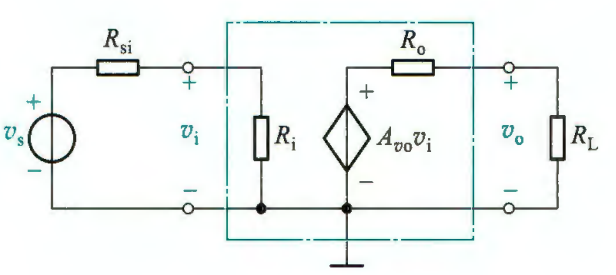
\includegraphics[width=0.5\linewidth]{pic/电压放大电路模型.png}
    \caption{电压放大电路模型\cite{康华光}\label{电压放大电路模型}}
\end{figure}

举一个简单的例子。图\ref{电压放大电路模型}为电压放大电路,其中$R_\mathrm{i}$为输入电阻,$R_\mathrm{o}$为输出电阻,则实际电压增益为
\begin{equation}
    A_v=A_{v\mathrm{o}}\frac{R_{\mathrm{L}}}{R_{\mathrm{L}}+R_{\mathrm{o}}}
\end{equation}

⼀个类似概念是\textbf{源放大倍数}:
\begin{equation}
    A_{v\mathrm{s}}=\frac{v_{\mathrm{o}}}{v_{\mathrm{s}}}=\frac{v_{\mathrm{o}}}{v_{\mathrm{i}}}\cdot \frac{v_{\mathrm{i}}}{v_{\mathrm{s}}}=A_v\frac{R_{\mathrm{i}}}{R_{\mathrm{si}}+R_{\mathrm{i}}}.
\end{equation}

由上面两个公式可知,当$R_\mathrm{i}=0,R_\mathrm{o}=\infty$时,可以避免负载电路对增益的影响以及信号在信号源上的衰减。因此,电压放大电路适用于信号源内阻较小而负载较大的情况,对其他三种类型的电路也可以进行类似的分析。

\section{放大电路的分析方法}
所谓的分析放大电路,本质上是去求解一个复杂的时变非线性方程(组),但这个方程(组)基本无法严格求解。在实际应用中,往往没有精确计算的必要,只要在设计误差范围内可以使用就行了。因此,人们提出了\textbf{图解法}\index{T!图解法}和\textbf{小信号模型法}\index{X!小信号模型法}来近似求解电路。两种方法在本质上都充分利用了“小信号”足够小的特点,类似于泰勒展开保留到一阶项,使得电路线性化,从而可以充分利用线性电路的分析方法。

在介绍这两种方法之前,先讲解一下放大电路通常进行的分解。

\subsection{直流通路和交流通路}
由放大电路的工作原理,放大电路中往往是直流量和交流量共存。其中直流分量往往用于提供工作点,使得三极管能够起到放大信号的作用,而交流分量才是真正被放大的部分。

此外,由于电路中有电容和电感的存在,直流量和交流量的流经的通路不同,因此需要引入直流通路和交流通路。这种思想类似于叠加定理,但值得注意的是,叠加定理仅对于线性电路成立,而此处的三极管为非线性元件。后面会看到,对于同样一个信号,由于放大电路的静态工作点不同,其对交流信号的放大倍数也不同,必须先求解静态工作点然后再做交流等效,这也能说明分解为直流通路和交流通路并非简单的叠加定理。

\subsubsection{一、直流通路}
\textbf{静态}\index{J!静态}是在放大电路没有输入信号时,电路中各处电压、电流都是不变的情况。而\textbf{直流通路}\index{Z!直流通路}是在直流电源作用下,直流电流流经的通路,用于对静态工作点的估算和对有源元件工作状态的判定。

对于直流通路,需要将电容视为开路,交流电源置零。

\subsubsection{二、交流通路}
\textbf{动态}\index{D!动态}是在放大电路存在输入信号后,电路中各处电压、电流都处于动态工作的情况。\textbf{交流通路}\index{J!交流通路}是交流输入信号下交流信号流经的通路,用于研究动态参数。

对于交流通路,需要将电容视为短路,直流电源置零(即电压源短路,电流源开路)。

\subsection{图解法}
图解法往往简单直观地反映了晶体管工作情况,但是必须实测所用管的特性曲线,且进行定量分析时误差较大。由于图解法有助于理解为什么说动态是建立在静态的基础上的,因此在此简单介绍。

\subsubsection{一、静态工作点的确定}
在输入回路中,Q点应当既在输入特性曲线上,又应满足外电路的回路方程。对于输出回路也类似。

直流通路下得到的直线方程,称为\textbf{直流负载线}\index{Z!直流负载线},其形式往往满足$v=V-iR$。

\subsubsection{二、动态工作参数的确定}
加入交流小信号以后,由于直流信号和交流信号流经的回路不同,相应的工作点会在Q点附近沿着\textbf{交流负载线}\index{J!交流负载线}振荡。此时负载线的不同往往是由于在交流情况下会多并上一个$R_\mathrm{L}$,因此交流负载线比直流负载线更陡。

\subsubsection{三、波形非线性失真的分析}
当Q点过低,当小信号的在负向时可能会导致元件截止,从而导致\textbf{截止失真}\index{S!失真!截止失真};而当Q点过高,当小信号的在正向时可能会导致元件饱和,从而导致\textbf{饱和失真}\index{S!失真!饱和失真}。

\subsection{小信号模型分析法}
在实际中,如果想使用图解法,首先需要知道元件的输入输出特性曲线,较麻烦。在工程上,通过建立小信号模型,往往可以将复杂的非线性电路的求解转化为简单的线性问题来处理。在放大电路中,输入信号为\textbf{低频小信号}的情况下,晶体管往往可以被看做是一个双口网络,因此可以引入\textbf{H参数小信号模型}\index{H!H参数小信号模型}。

\subsubsection{一、BJT的H参数小信号模型}
BJT的H参数小信号模型如图\ref{BJT的简化小信号模型}所示,其中
\begin{equation}\label{公式-BJT的小信号模型}
    r_{\mathrm{be}}=r_{\mathrm{bb'}}+(1+\beta)\frac{V_\mathrm{T}}{I_{\mathrm{EQ}}}\approx\qty{200}{\ohm}+(1+\beta)\frac{\qty{26}{mV}}{I_{\mathrm{EQ}}},
\end{equation}
其中$V_\mathrm{T}$为电压当量。

\begin{figure}[htb]
    \centering
    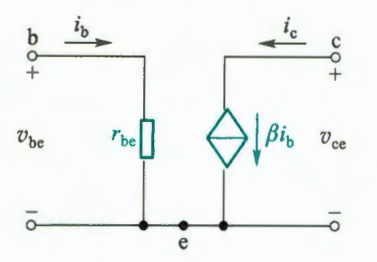
\includegraphics[width=0.3\linewidth]{pic/BJT的简化小信号模型.png}
    \caption{BJT的简化小信号模型\cite{康华光}\label{BJT的简化小信号模型}}
\end{figure}

\subsubsection{二、N型MOSFET的H参数小信号模型}
\textit{(本小节的内容仅做了解)}

NMOS的H参数小信号模型如图\ref{NMOS的简化小信号模型}所示,其中
\begin{equation}
    r_{\mathrm{ds}}\approx\frac{1}{\lambda i_{\mathrm{DQ}}}, g_\mathrm{m}=2\sqrt{K_{\mathrm{n}}i_{\mathrm{DQ}}},
\end{equation}
其中的参数$\lambda$来自沟道长度调制效应,实际中往往取$\lambda=0$。

\begin{figure}[htb]
    \centering
    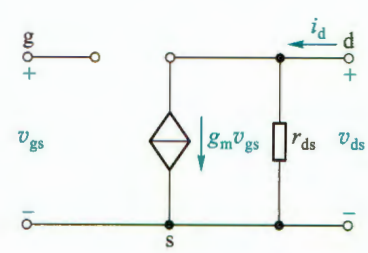
\includegraphics[width=0.3\linewidth]{pic/NMOS的简化小信号模型.png}
    \caption{NMOS的简化小信号模型\cite{康华光}\label{NMOS的简化小信号模型}}
\end{figure}

\subsubsection{三、利用小信号模型对放大电路的分析}
利用小信号模型分析放大电路的方法往往比较固定,一般情况下,按照固定的套路都能够解决问题。本节以BJT管为例,介绍如何利用小信号模型分析放大电路的基本套路。

\textbf{1.静态分析:}

\begin{itemize}
    \item 将电路中电容视为断路;
    \item 将BJT的发射结按照恒压降模型计算(对于硅管$V_{\mathrm{B}}-V_{\mathrm{E}}=\qty{0.7}{V}$);
    \item 寻找电压路径,使得该路径两端电压确定,且其中仅存在电阻和三极管(基极到发射极),并计算$I_{\mathrm{BQ}}$或者$I_{\mathrm{CQ}}$;
    \item 寻找电流路径,使得该路径两端电压确定,且其中仅存在电阻和三极管(集电极到发射极),并计算$V_{\mathrm{CEQ}}$。
\end{itemize}

\textbf{2.动态分析:}

\begin{itemize}
    \item 判断元件工作状态是否进入放大区;
    \item 利用三级管的$I_{\mathrm{EQ}}$计算动态参数$r_{\mathrm{be}}$;
    \item 将大电容(耦合电容和旁路电容)视为短路,直流信号源置零,并将三极管替换为小信号模型,计算所需要的结果。
\end{itemize}

\subsection{共射放大电路的分析}
本节通过两种不同的共射放大电路作为例题来介绍如何使用图解法和小信号模型法。

\subsubsection{一、图解法求解基本共射放大电路}

基本共射放大电路如图\ref{基本共射放大电路}所示,其中$v_{\mathrm{s}}$为待放大的时变输入信号。假设参数使BJT工作在放大区。

\begin{figure}[htb]
    \centering
    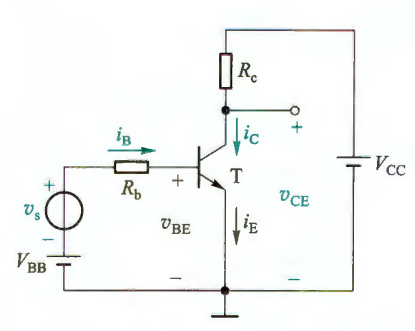
\includegraphics[width=0.55\linewidth]{pic/基本共射放大电路.png}
    \caption{基本共射放大电路\cite{康华光}\label{基本共射放大电路}}
\end{figure}

\textbf{1.静态工作点的分析}

由于电路中交流量叠加在直流量上,因此先考虑直流通路。令$v_{\mathrm{s}}=0$,则输入端的外电路特性曲线为$v_{\mathrm{BE}}=V_{\mathrm{BB}}-i_{\mathrm{B}}R_{\mathrm{b}}$。与输入特性曲线联立就能得到静态工作点Q以及电流$I_{\mathrm{BQ}}$。

类似地,在输出特性曲线上,画出$v_{\mathrm{CE}}=V_{\mathrm{CC}}-i_{\mathrm{C}}R_{\mathrm{c}}$,与$i_{\mathrm{B}}=I_{\mathrm{BQ}}$对应的特性曲线的交点就是静态工作点Q。

\begin{figure}[htb]
    \centering
    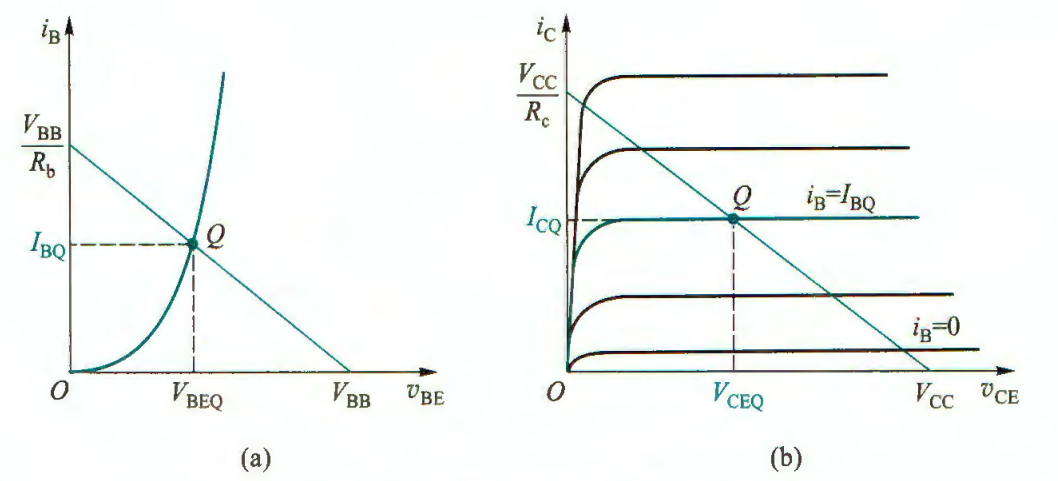
\includegraphics[width=0.8\linewidth]{pic/静态工作点的图解分析.png}
    \caption{静态工作点的图解分析\cite{康华光}\label{静态工作点的图解分析}}
\end{figure}

\textbf{2.动态参数的分析}

当$v_{\mathrm{s}}=V_{\mathrm{sm}}\sin \omega t$时,输入负载曲线为$v_{\mathrm{BE}}=V_{\mathrm{BB}}+v_{\mathrm{s}}-i_{\mathrm{B}}R_{\mathrm{b}}$,画出图像如图\ref{动态工作情况的图解分析1}所示,可以读出$i_{\mathrm{B}}$的波形。

类似地,可以在输出特性曲线上求出其他参数,如图\ref{动态工作情况的图解分析2}所示。

\begin{figure}[htb]
    \centering
        \subcaptionbox{输入回路\cite{康华光}\label{动态工作情况的图解分析1}}
        {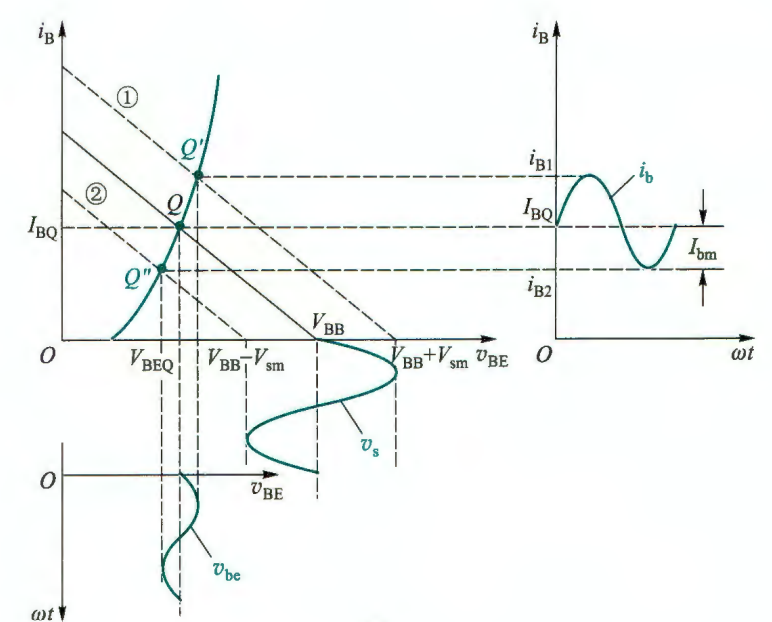
\includegraphics[width=0.45\textwidth]{pic/动态工作情况的图解分析1.png}}\qquad
        \subcaptionbox{输出回路\cite{康华光}\label{动态工作情况的图解分析2}}
        {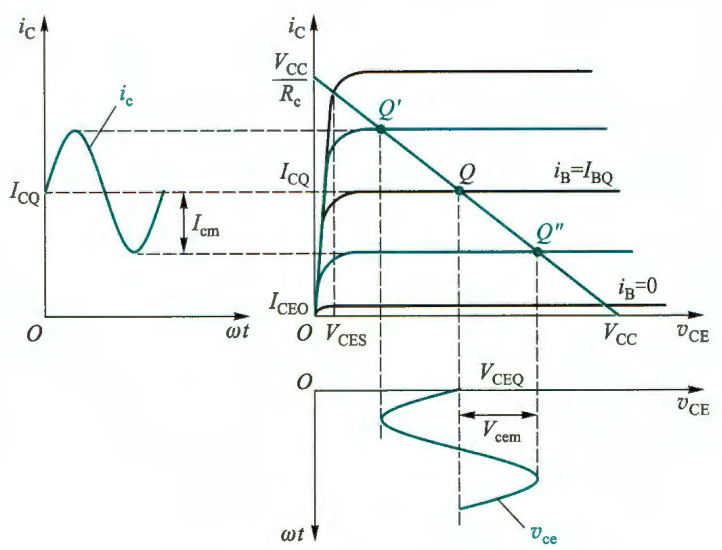
\includegraphics[width=0.45\textwidth]{pic/动态工作情况的图解分析2.png}}
        \caption{动态工作情况的图解分析\label{动态工作情况的图解分析}}
\end{figure}

\subsubsection{二、小信号模型法求解基极分压式射极偏置共射放大电路}

基极分压式射极偏置共射放大电路如图\ref{基极分压式射极偏置共射放大电路-电路图}所示。其中参数的选取需要使得电路满足$i_2\gg i_{\mathrm{B}}$,因此$i_1\approx i_{\mathrm{2}}$。

同时,选取合适的$R_{\mathrm{b1}}$、$R_{\mathrm{b2}}$和$R_{\mathrm{c}}$使得BJT工作在放大区。

\begin{figure}[htb]
    \centering
        \subcaptionbox{电路图\cite{康华光}\label{基极分压式射极偏置共射放大电路-电路图}}
        {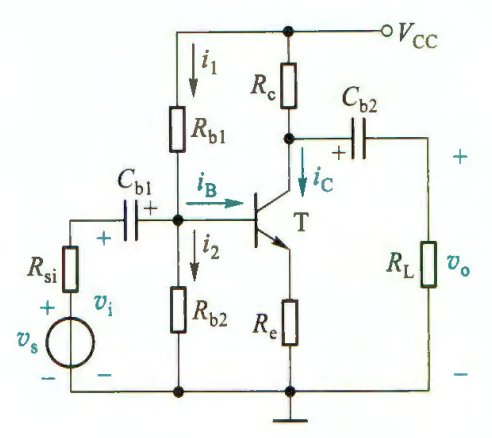
\includegraphics[width=0.4\textwidth]{pic/基极分压式射极偏置共射放大电路-无射极旁路电容.png}}\qquad
        \subcaptionbox{直流通路\cite{康华光}\label{基极分压射极偏置电路-直流通路}}
        {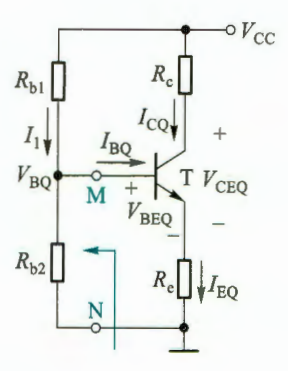
\includegraphics[width=0.28\textwidth]{pic/基极分压射极偏置电路-直流通路.png}}
        \caption{基极分压式射极偏置共射放大电路\label{基极分压式射极偏置共射放大电路}}
\end{figure}

\textbf{1.静态分析:}

断开$C_{\mathrm{b1}}$、$C_{\mathrm{b2}}$支路,得到图\ref{基极分压射极偏置电路-直流通路}。由于$i_1\approx i_{\mathrm{2}}$,因此
\begin{equation}
    V_{\mathrm{BQ}}=\frac{R_{\mathrm{b2}}}{R_{\mathrm{b1}}+R_{\mathrm{b2}}}V_{\mathrm{CC}}
\end{equation}

由此在经过基极b、发射极e和电阻$R_\mathrm{e}$的支路上,可以计算出
\begin{equation}
    I_{\mathrm{BQ}}=\frac{V_{\mathrm{BQ}}-V_{\mathrm{BEQ}}}{(1+\beta)R_{\mathrm{e}}}
\end{equation}

再代入\ref{公式-BJT的小信号模型}式,就能计算出小信号模型中的$r_\mathrm{be}$。

\textbf{2.动态分析:}

将所有电容短路,直流信号源置零,并将三极管替换为小信号模型,就能得到图\ref{基极分压射极偏置电路-交流通路}。

\begin{figure}[htb]
    \centering
    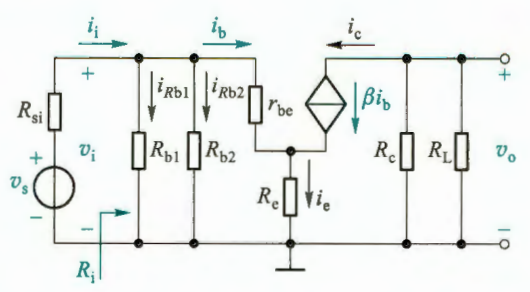
\includegraphics[width=0.5\linewidth]{pic/基极分压射极偏置电路-交流通路.png}
    \caption{基极分压式射极偏置共射放大电路的交流通路\cite{康华光}\label{基极分压射极偏置电路-交流通路}}
\end{figure}

因为有
\begin{align}
    v_\mathrm{o}=-\beta i_\mathrm{b} (R_\mathrm{c}\parallel R_\mathrm{L}) \\
    v_\mathrm{i}=(r_\mathrm{be}+(1+\beta)R_\mathrm{e})i_\mathrm{b}
\end{align}
所以电压增益为
\begin{equation}\label{公式-共射放大电路增益}
    A_v=\frac{v_\mathrm{o}}{v_\mathrm{i}}=-\frac{\beta (R_\mathrm{c}\parallel R_\mathrm{L})}{r_\mathrm{be}+(1+\beta)R_\mathrm{e}}
\end{equation}

对于输入电阻
\begin{equation}
    R_\mathrm{i}=R_\mathrm{b1} \parallel R_\mathrm{b2} \parallel (r_\mathrm{be}+(1+\beta)R_\mathrm{e})
\end{equation}

在计算输出电阻时,本身并没有电源在起作用。此时应该把将原来的独立源直接置零,并把输出网络的负载换成一个电源。在BJT电路中,$r_\mathrm{ce}$往往很大,因此上述电路的输出电阻
\begin{equation}
    R_\mathrm{o}=R_\mathrm{c}
\end{equation}

\section{BJT的三种基本放大电路}
晶体管组成的基本放大电路是由共射、共基、共集三种接法。要判断某个放大电路属于哪种类型,先判断输⼊和输出分别是哪⼀极,然后剩下那一极就是共什么极,如图\ref{BJT放大电路三种组态的性能}所示。

\begin{figure}[htb]
    \centering
    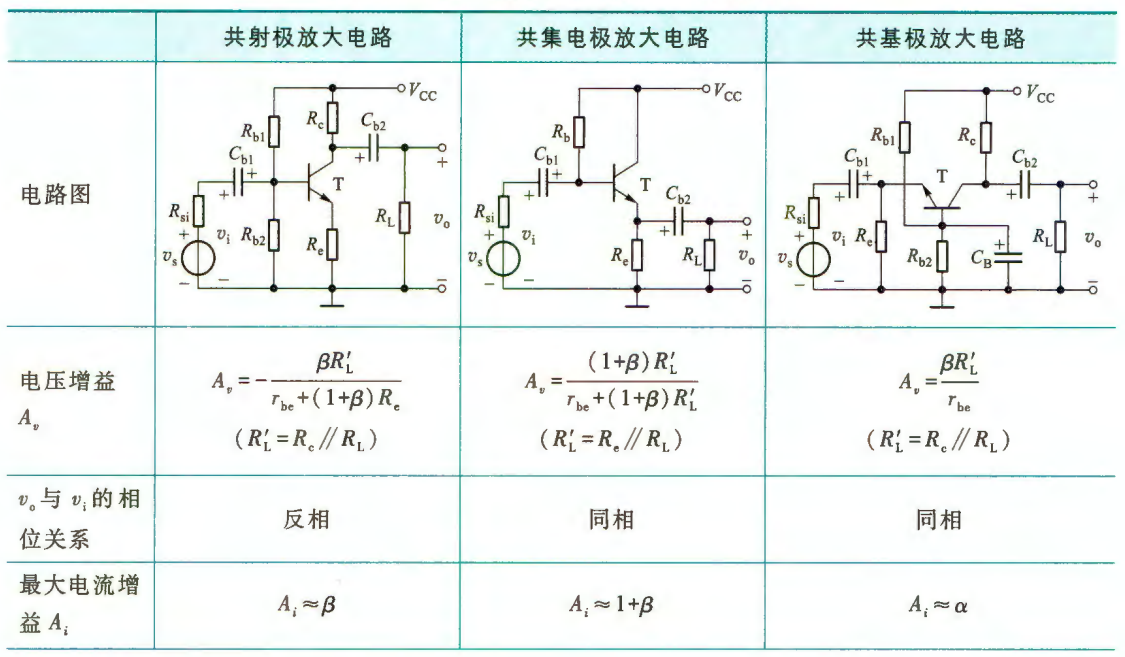
\includegraphics[width=0.9\linewidth]{pic/BJT三种类型的放大电路-1.png}
    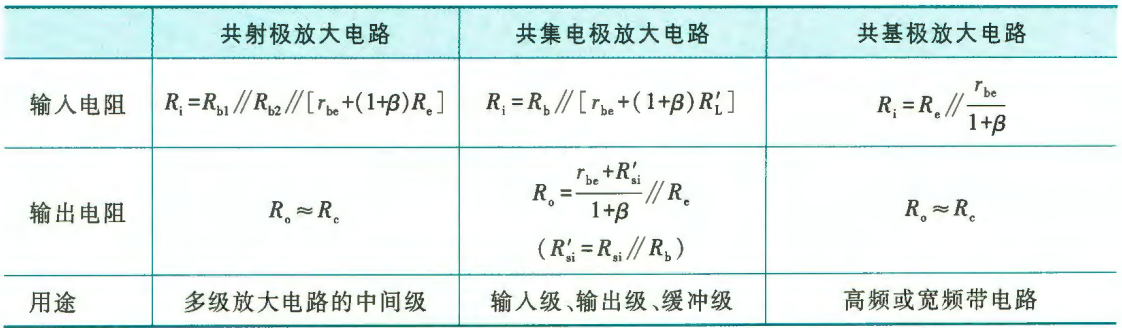
\includegraphics[width=0.9\linewidth]{pic/BJT三种类型的放大电路-2.png}
    \caption{BJT放大电路三种组态的性能\cite{康华光}\label{BJT放大电路三种组态的性能}}
\end{figure}

当掌握基本分析方法后,可以通过对这三种电路的分析加深印象。由于教材5.2.4节和5.2.5节有详细的推导,此处从略,仅提供基本结论。

1.基本共射放大电路既能放大电流又能放大电压,常作为低频放大电路的单元电路。

2.基本共集放大电路只能放大电流不能放大电压,输入电阻大,输出电阻小,有电压跟随的特点。

3.基本共基放大电路只能放大电压不能放大电流,有电压跟随的特点。